\label{sec:results}

All numbers below are paired against the dense baseline of
Proposition~\ref{prop:reduction} on identical queries, with cluster-bootstrap intervals.
Ledger identifiers index \texttt{docs/10\_EXPERIMENT\_LEDGER.md}.

\subsection{Completion: descent beats cosine, and loses to a plain classifier}
\label{sec:completion}

\begin{table}[t]\centering\small
\caption{The image study with its matched baseline. The metric is \textbf{same-class top-1
accuracy} over ten classes, not identification, and the cue's source image is \emph{not} in
the bank --- see \S\ref{sec:occlusion}. $\beta$, $k$ and $\tau$ all selected on the same
disjoint tune half; one pre-committed paired test on the held-out half. $n{=}5{,}847$ query
instances from $1{,}949$ distinct images; bootstrap resamples images. $^{*}$CI excludes zero.}
\label{tab:images}
% GENERATED by scripts/make_tables.py -- do not edit
\begin{tabular}{@{}lrrrl@{}}
\toprule
\textbf{Occlusion} & \textbf{Cosine} & \textbf{Descent} ($\beta{=}40$) & \textbf{$k$-NN vote} ($k{=}20$) & \textbf{Descent $-$ vote (95\% CI)} \\
\midrule
30\% & 0.730 & 0.733 & 0.761 & $-0.028$ \ci{-0.040}{-0.017}$^{*}$ \\
50\% & 0.542 & 0.559 & 0.600 & $-0.041$ \ci{-0.054}{-0.027}$^{*}$ \\
70\% & 0.386 & 0.407 & 0.445 & $-0.038$ \ci{-0.052}{-0.024}$^{*}$ \\
\midrule
\textbf{pooled} & \textbf{0.553} & \textbf{0.566} & \textbf{0.602} & $\mathbf{-0.036}$ \ci{-0.043}{-0.028}$^{*}$ \\
\bottomrule
\end{tabular}

\end{table}

\begin{table}[t]\centering\small
\caption{Completion as the premise defines it (\xid{X113b}): cues are occluded copies of
images that \emph{are} in the bank, scored by \textbf{same-image} recall@1. Identity control
at $0\%$ occlusion: cosine recall@1 $=1.0000$. $\beta$ selected on a disjoint half of the
bank images and used once; selection chose $\beta{=}80$, the top of the grid. Same-class
accuracy on the identical cues is shown for comparison with Table~\ref{tab:images}.}
\label{tab:completion}
% GENERATED by scripts/make_tables.py -- do not edit
\begin{tabular}{@{}lrrlrrr@{}}
\toprule
& \multicolumn{3}{c}{\textbf{Same-image recall@1}} & \multicolumn{3}{c}{\textbf{Same-class accuracy}} \\
\cmidrule(lr){2-4}\cmidrule(lr){5-7}
\textbf{Occlusion} & Cosine & Descent & $\Delta$ (95\% CI) & Cosine & Descent & $\Delta$ \\
\midrule
30\% & 0.855 & 0.855 & $+0.000$ \ci{+0.000}{+0.000} & 0.915 & 0.915 & $+0.000$ \\
50\% & 0.635 & 0.630 & $-0.005$ \ci{-0.015}{+0.000} & 0.755 & 0.760 & $+0.005$ \\
70\% & 0.380 & 0.375 & $-0.005$ \ci{-0.015}{+0.000} & 0.545 & 0.535 & $-0.010$ \\
\midrule
\textbf{pooled} & \textbf{0.623} & \textbf{0.620} & $\mathbf{-0.003}$ \ci{-0.008}{+0.000} & 0.738 & 0.737 & $-0.002$ \\
\bottomrule
\end{tabular}

\end{table}

Table~\ref{tab:images} was for most of this project the paper's one clean positive for the
energy mechanism itself, and the first three columns are unchanged from that version:
descent beats cosine by $+0.014$ pooled, growing with corruption severity, on a
pre-committed held-out split. The fourth column is why we no longer report it that way. A
soft $k$-NN class vote --- selected on the same tune half, from a grid declared in advance
--- scores $0.602$ where descent scores $0.566$, and beats descent at every occlusion
level. \S\ref{sec:occlusion} gives the mechanism: on a \emph{class} metric, descent at
$\beta{=}40$ is an implicit class vote over $\approx 13$ neighbours, and an explicit vote
over $k{=}20$ does the same job better. Table~\ref{tab:completion} then asks the question
the metric name implied all along --- can descent retrieve the \emph{particular} stored
image a cue was degraded from --- and the answer is $-0.003$ \ci{-0.008}{+0.000}.

The latency comparison is unchanged and now lands differently: descent costs $21\times$
cosine's wall-clock latency ($0.0502$\,ms vs.\ $0.0024$\,ms per query) to be beaten by a
classifier that costs one extra argpartition.

Two further qualifications, which predate \xid{X113} and survive it. First, the apparent
advantage is \emph{capacity-dependent}: growing the bank from $100$ to $4{,}000$ patterns at
fixed $\beta{=}32$, cosine overtakes descent past $N\approx 800$. Second, descent's rank-1
gain over cosine comes with a \emph{shortlist regression}: recall@5 is $0.605$ against cosine's $0.759$
and MRR $0.589$ against $0.643$, all class-level (Table~\ref{tab:multibeta}). Converging to a single
attractor means ranks 2--5 measure proximity to that attractor rather than to the query,
which is Remark~\ref{rem:shortlist} and is now confirmed in three independent settings.

\paragraph{Two earlier verdicts of ours, withdrawn.} A previous version of this study used
$80$ distinct images with unpaired intervals roughly $5\times$ the effect size and $\beta$
tuned on the test images; those conclusions were underpowered and Table~\ref{tab:images}
supersedes them. The version that replaced it --- the one with the honest split, which we
described as a clean positive for the energy mechanism --- is withdrawn in turn by its own
fourth column. The number stands; the interpretation does not.

\subsection{Semantic match: every increment of descent costs accuracy}
\label{sec:semantic}

\begin{table}[t]\centering\small
\caption{\textsc{LoCoMo}, $1{,}977$ questions over $5{,}882$ turns. \texttt{anchor}
interpolates between pure cosine ($1.0$) and pure descent ($0.0$); the baseline is a point in
our own parameter space, so the sweep measures exactly what descent adds. The reduction check
passes $196/196$ at $\texttt{anchor}{=}1.0$.}
\label{tab:locomo}
% GENERATED by scripts/make_tables.py -- do not edit
\begin{tabular}{@{}lrl@{}}
\toprule
\textbf{Condition} & \textbf{Coverage@5} & \textbf{95\% CI} \\
\midrule
\textbf{$\texttt{anchor}{=}1.00$ \textit{(is cosine)}} & \textbf{0.336} & \ci{0.316}{0.355} \\
$\texttt{anchor}{=}0.90$, $\mathrm{pp}_0{=}32$ & 0.331 & \ci{0.311}{0.351} \\
$\texttt{anchor}{=}0.75$, $\mathrm{pp}_0{=}4$ & 0.321 & \ci{0.301}{0.340} \\
$\texttt{anchor}{=}0.50$, $\mathrm{pp}_0{=}4$ & 0.304 & \ci{0.285}{0.324} \\
$\texttt{anchor}{=}0.25$, $\mathrm{pp}_0{=}4$ & 0.273 & \ci{0.255}{0.292} \\
$\texttt{anchor}{=}0.00$, $\mathrm{pp}_0{=}4$ & 0.252 & \ci{0.234}{0.271} \\
energy, fixed $\beta{=}32$ & 0.236 & \ci{0.218}{0.254} \\
\bottomrule
\end{tabular}

\end{table}

Table~\ref{tab:locomo} is monotone: the optimum sits at the boundary where the method
\emph{is} the baseline. The table shows the best $\mathrm{pp}_0$ at each anchor; the worst
cell of the full sweep is $\texttt{anchor}{=}0.00,\ \mathrm{pp}_0{=}32$ at $0.201$
\ci{0.184}{0.218}, which is the broad-start annealing failure of \S\ref{sec:band} compounding
with the absent query anchor. There is no interior operating point at which descent helps on
question$\to$evidence retrieval, which is the dominant query type in deployed agent memory.

\paragraph{A data bug that invalidated an earlier result.} \textsc{LoCoMo} dialogue
identifiers are unique only \emph{within} a conversation: $5{,}882$ turns carry $1{,}033$
distinct identifiers, and $132$ of conversation~0's $134$ gold identifiers recur in other
conversations. Our first capacity sweep pooled banks without namespacing, so distractors
satisfied gold identifiers and scored as hits. Its headline---``adaptive $\beta$ improves as
the bank grows''---was an artefact; with namespaced identifiers adaptive $\beta$ \emph{degrades}
($0.250 \to 0.231$), merely less steeply than fixed $\beta$ ($0.244 \to 0.216$). We report
this because the failure mode is specific to this widely used benchmark and will recur.

\subsection{Composition: the one mechanism that works}
\label{sec:composition}

\paragraph{The gate.} Before building a predictor we checked whether cosine already solves
``what happened next''. It does not: Recall@1 is $0.105$ with the gold episode at median rank
$24$ of $1{,}319$. The failures are instructive---they are lexical collisions across
unrelated storylines, where a cue about a cottage drive returns ``forty minutes each way''
from an apartment-hunting thread. Oracle-restricting candidates to the correct storyline
still reaches only $0.488$, so the difficulty is not merely retrieval breadth. Temporal
succession is genuinely not a similarity relation (\xid{X16}).

\paragraph{The parametric predictor fails completely.} A low-rank JEPA predictor fitted on
some storylines and evaluated on others reaches Recall@1 of $1.000$ on the storylines it was
fitted on and $0.000$ on unseen ones, against the cosine baseline's $0.131$---worse
than doing nothing. No capacity escapes it: across ranks $2$ to $32$ the best unseen
Recall@1 at any setting is $0.016$, and the two largest capacities score exactly zero.
The diagnostic explains why: displacement vectors between consecutive episodes are
near-orthogonal (mean pairwise cosine $+0.004$) and the top ten principal
components carry only $31\%$ of their variance. There is no global ``and then''
direction to fit, and $134$ transitions in $768$ dimensions cannot teach one
(\xid{X17}, re-run as \xid{X17-r}). We report this as a result about inductive bias, not as
a tuning failure.

\paragraph{The nonparametric predictor works, on our corpus and on a public one.}
Equation~\eqref{eq:knnwm}, with $(k,\tau)$ selected on held-out storylines or sessions only,
beats cosine on one-hop association in three independent implementations
(Table~\ref{tab:assoc}). The third is the one that matters: it runs the same probe design on
\textsc{LoCoMo}, a benchmark built by another group, against the \emph{full pooled bank} of
$5{,}882$ turns from all ten conversations, so a prediction must beat distractors from nine
unrelated conversations as well as its own. Dialogue identifiers are namespaced by
conversation---without that, $5{,}882$ turns carry only $1{,}033$ distinct identifiers and
distractors satisfy gold identifiers, the bug described in \S\ref{sec:semantic}.

\begin{table}[t]\centering\small
\caption{One-hop temporal association. Three implementations, two corpora. ``Clusters'' is
the bootstrap resampling unit---storylines for the episodic corpus, sessions for
\textsc{LoCoMo}. Implementations (ii) and (iii) were written without reference to (i).
Absolute scores are lower on \textsc{LoCoMo} because the task is harder: a larger pooled
bank, nine conversations of distractors, and speaker-alternating turns. The relative effect
is \emph{larger} there.}
\label{tab:assoc}
% GENERATED by scripts/make_tables.py -- do not edit
\footnotesize\setlength{\tabcolsep}{4pt}
\begin{tabular}{@{}llrrccl@{}}
\toprule
& \textbf{Corpus} & \textbf{Probes} & \textbf{Clust.} & \textbf{Cosine} & \textbf{WM} & \textbf{Paired $\Delta$ R@1} \\
\midrule
(i) & episodic (ours), 50/50 & 123 & 61 & 0.106 & 0.130 & $+0.024$ \ci{-0.032}{+0.083}, $p{=}0.24$ \\
(ii) & episodic (ours), 4-fold & 257 & 122 & 0.105 & 0.140 & $+0.035$ \ci{+0.012}{+0.061}, $p{=}0.002$ \\
(iii) & \textbf{\textsc{LoCoMo}}, 4-fold & \textbf{5,233} & \textbf{272} & \textbf{0.064} & \textbf{0.107} & $\mathbf{+0.043}$ \ci{+0.036}{+0.050}, $\mathbf{p<10^{-4}}$ \\
\bottomrule
\end{tabular}

\end{table}

\begin{figure}[t]\centering
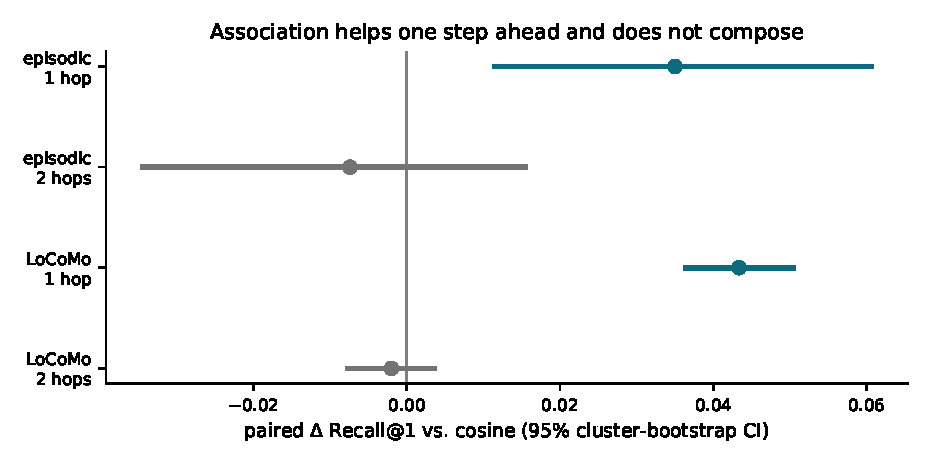
\includegraphics[width=0.78\textwidth]{figures/assoc_hops.pdf}
\caption{Paired $\Delta$ Recall@1 against cosine, both corpora, one and two hops. Intervals
are 95\% cluster bootstrap (storylines for the episodic corpus, sessions for
\textsc{LoCoMo}). The one-hop effect is positive on both corpora and larger on the public,
harder one; the two-hop effect is null on both. Generated by
\texttt{scripts/make\_tables.py}.}
\label{fig:hops}
\end{figure}

On \textsc{LoCoMo} the effect is $+67\%$ relative at Recall@1 and $+0.077$
\ci{+0.067}{+0.087} at Recall@5 ($0.174 \to 0.251$). This is the only claim in the paper with
external validity, and the only one reproduced three times; we weight it accordingly, and we
have restricted the paper's positive claims to it.

\paragraph{Multi-hop composition does not hold. We withdraw our own earlier result.}
An earlier run of ours indicated that iterating the predictor recovers two-hop chains it was
never trained on: Recall@5 of $0.446$ against cosine's $0.262$, $\Delta = +0.185$
\ci{+0.076}{+0.297}, $p<0.001$. That was the strongest result we had recorded. It does not
survive.

Three subsequent measurements (Table~\ref{tab:twohop}) return nulls, the last of them on
public data at $n{=}5{,}013$ with $272$ clusters---roughly $37\times$ the probe count of the
original. We therefore withdraw the two-hop claim as an artifact rather than suspending it.
The $+0.185$ figure should not be cited, including from our own ledger, where it now carries
a pointer to this result.

\begin{table}[t]\centering\small
\caption{Two-hop composition, every measurement we have. The original script was lost before
it was committed, so (a) cannot be re-run; (b) and (c) are independent reimplementations
under storyline- and session-disjoint rotation. Row (c) is $p{=}0.77$; the claim is withdrawn.}
\label{tab:twohop}
% GENERATED by scripts/make_tables.py -- do not edit
\footnotesize\setlength{\tabcolsep}{4pt}
\begin{tabularx}{\textwidth}{@{}l>{\raggedright\arraybackslash}X rc>{\raggedright\arraybackslash}X@{}}
\toprule
& \textbf{Corpus / protocol} & \textbf{Probes} & \textbf{Metric} & \textbf{Result} \\
\midrule
(a) & episodic, 50/50 \textit{(lost)} & 65 & R@5 & $0.446$ vs.\ $0.262$; $\Delta{+}0.185$ \\
(b) & episodic, 4-fold & 135 & R@5 & $0.230$ vs. $0.207$; spans zero \\
(c) & \textsc{LoCoMo}, 4-fold & 5,013 & R@1 & $0.041$ vs. $0.043$; $\Delta-0.002$ \ci{-0.008}{+0.004} \\
\bottomrule
\end{tabularx}

\end{table}

A residual signal does exist at two hops on \textsc{LoCoMo} at Recall@5 ($+0.012$
\ci{+0.004}{+0.019}), an order of magnitude below the one-hop effect and not visible at
Recall@1. We report it for completeness and do not build on it. The honest summary is that
association helps one step ahead and does not compose: the error introduced by predicting
from a prediction exceeds whatever compositional signal the second step carries.

\paragraph{Why we report this at length.} The withdrawn result was, for several weeks, the
headline of this project and the organising claim of a design document built on top of it.
It was overturned by reimplementation, not by review---twice---and the version that finally
settled it is the public-benchmark run that a reviewer would have demanded anyway. We regard
the sequence as the strongest available evidence for \S\ref{sec:protocol}'s argument that
independent reimplementation is a distinct and stronger property than peer inspection.

\subsection{Eight mechanisms that do not pay for themselves}
\label{sec:negatives}

\begin{table}[t]\centering\small
\caption{Negative results, each with its diagnosed mechanism. ``Regime'' indicates where the
test was run. Two of these overturn claims we previously made ourselves.}
\label{tab:negatives}
\begin{tabular}{@{}p{0.235\textwidth}p{0.20\textwidth}p{0.45\textwidth}@{}}
\toprule
\textbf{Mechanism} & \textbf{Result} & \textbf{Diagnosed mechanism} \\
\midrule
Multi-step descent (G1) & no effect & Identical to one step above the $\beta$ threshold---precisely what Corollary~\ref{cor:degeneracy} predicts. Once $\beta$ commits on step one there is nothing left to do (\xid{X2}). \\
Residual peeling & $0.268$ vs.\ repulsion $0.290$ & Restores multi-answer recall on orthogonal synthetic patterns ($0.258 \to 1.000$) and inverts on real embeddings: non-orthogonal golds mean projecting one out damages the others (\xid{X5}, \xid{X13}). \\
Repulsive parallel descent & $+0.004$, $p{=}0.43$ & Survives to $146$ questions but not to held-out selection. The $+0.042$ trend was hyperparameter overfitting (\xid{X15}). \\
Noise-seeded parallel descent & fails at every $\sigma$ & No intermediate value exists. Too little noise and all chains land in one basin; too much and they scatter uniformly, where correct answers are no likelier than any others. Isotropic noise carries no information about where the other answers are (\xid{X7}). \\
Cosine-seeded parallel descent & exactly chance & Circular. Stored patterns are exact fixed points, so descent is a no-op; ranking the landing sites requires a signal the descent has already destroyed. Ranking them by similarity to the cue scores $1.000$---but that ranking \emph{is} cosine top-$k$ (\xid{X7}). \\
Multi-scale $\beta$ & $+0.0003$ \ci{-0.0014}{+0.0021} & Expressively distinct and performance-neutral. An integrated mixture is provably not reducible to any single $\beta$ \citep{yang2018softmax}, and diverges from an ensemble at $T{=}8$ ($63\%$ top-1 agreement), yet changes \emph{which} queries are answered, not how many (\texttt{exp\_multibeta\_scales.py}; this study predates the ledger and has no \xid{X} identifier). \\
Per-memory / learned $\beta$ & inert & The learned values ($51$--$88$) land above the leverage band, and a shuffle control with the same values randomly reassigned scores identically. Conditioning $\beta$ on the query is motivated---the optimum does differ by corruption level---but the learned function converged to a near constant ($\beta{\approx}31$ everywhere). \\
Predictor coupled into the energy & never exceeds external & Interpolating the routing operator inside the descent step gives $0.130$ at $\eta{=}0.5$ and $0.154$ at $\eta{=}1.0$---the latter merely \emph{recovering} the external predictor, since $\eta{=}1$ replaces the Hopfield step entirely (\xid{X18}). This was our stated novelty against prior work \citep{dury2026pam} and it is withdrawn. \\
\bottomrule
\end{tabular}
\end{table}

\begin{table}[t]\centering\small
\caption{Multi-$\beta$ scales on the image task, with compute, ordered by top-1 accuracy.
As in Table~\ref{tab:images} the metric is \textbf{same-class} over ten classes --- which is
why the collapsed control sits at exactly $1/10$ --- so every row here inherits the matched
baseline of \S\ref{sec:occlusion} and none of them is compared against the $k$-NN vote.
Bootstrap resamples images. Controls were pre-registered to collapse and did. Note the
R@5/MRR columns: descent's shortlist is substantially worse than cosine's at every setting,
which is the shortlist regression of \S\ref{sec:completion} and Remark~\ref{rem:shortlist}.
Single $\beta$ beats cosine by $+0.0130$ \ci{+0.0074}{+0.0186}; no mixture beats single
$\beta$, and the vote of Table~\ref{tab:images} beats all of them.}
\label{tab:multibeta}
% GENERATED by scripts/make_tables.py -- do not edit
\footnotesize\setlength{\tabcolsep}{4pt}
\begin{tabular}{@{}lrrrrl@{}}
\toprule
\textbf{Condition} & \textbf{R@1} & \textbf{R@5} & \textbf{MRR} & \textbf{matmuls} & \textbf{$\Delta$ vs.\ single $\beta$} \\
\midrule
integrated mixture [32,40,48] & 0.559 & 0.591 & 0.584 & 16 & $+0.0036$ \ci{-0.0033}{+0.0106} \\
ensemble [32,40,48] & 0.559 & 0.599 & 0.586 & 48 & $+0.0032$ \ci{-0.0038}{+0.0103} \\
single beta=56 & 0.555 & 0.605 & 0.589 & 16 & --- \\
cosine & 0.542 & 0.759 & 0.643 & 1 & --- \\
\textit{control} ensemble [1,5,20] & 0.282 & 0.296 & 0.303 & --- & collapse (predicted) \\
\textit{control} integrated [1,5,20] & 0.108 & 0.318 & 0.217 & --- & collapse (predicted) \\
\bottomrule
\end{tabular}

\end{table}

Two findings survive from the controls in Table~\ref{tab:multibeta}. The integrated
$[1,5,20]$ control collapsed to exact chance ($0.108 = 1/10$) with \emph{identical} accuracy
at every occlusion level: one bad scale inside a shared trajectory poisons the entire state.
The ensemble version of the same scales reaches $0.282$, because there a bad scale only
dilutes one vote among independent runs. This is direct evidence that the coupling between
scales is real and can hurt as easily as it can fail to help.

\subsection{The multi-modality result, and why it does not help}
\label{sec:modes}

The predictor of Equation~\eqref{eq:knnwm} returns a weighted average. A natural hypothesis,
and one we committed to in a design document before testing it, is that this is a mistake:
if a cue has several legitimate successors, their average is a point in embedding space where
nothing is stored---a ridge between basins rather than a basin. Preserving the modes should
therefore help, and should motivate a stochastic (Boltzmann) rather than deterministic
relaxation \citep{ackley1985boltzmann,welling2011sgld}.

The premise is correct. Among the top three modes of $P(\cdot\mid q)$ the mean mutual cosine
is $0.353$, and $97\%$ of cues have modes that mutually disagree (\xid{X24}). There is
genuinely a distribution for averaging to destroy.

The conclusion is wrong. With step size matched (\S\ref{sec:method}), the mixture readout
\[
\mathrm{score}(m) \;=\; \lse_s\!\big[\beta\langle \xib_s, z_m\rangle + \log w_s\big]
\]
\emph{loses} to the averaged predictor at one hop, $\Delta = -0.062$ \ci{-0.094}{-0.034}, and
ties at two (\xid{X25}). The off-manifold gap the hypothesis rested on is also much smaller than assumed:
mean nearest-neighbour cosine is $0.482$ for a real stored episode against $0.462$ for an
averaged prediction, a gap of $-0.021$.

The mechanism is the step size. Averaging does two things at once, and the one that matters
is not the one the hypothesis named: it shrinks the displacement by a factor of $0.34$
through cancellation among near-orthogonal transitions, and that shrinkage keeps the cue in
control of where the prediction lands. Preserving the modes removes the shrinkage. On this
data, averaging is not a failure to be fixed---it is what makes the predictor work.

\paragraph{A later measurement sharpens this, and the invariant turns out to be about the
wrong comparison.} The step-size account above predicts that where there is no displacement
to shrink, the result should flip. We tested that in the modality where descent appeared to
win, with a
cue that is a degraded copy of two stored patterns at once (the spliced images of
\S\ref{sec:occlusion}) and hypotheses that are the cue plus stored vectors rather than
displacements, so no step size is in play. It flips, decisively: logsumexp beats averaging
in $20$ of $21$ $(K_0,\beta)$ cells with intervals excluding zero, by $+0.178$
\ci{+0.152}{+0.205} at the cell selected on a disjoint half (\xid{X111}). The gap widens
with $\beta$ because the averaged combiner collapses onto its heaviest mode and throws the
cue away, while logsumexp degrades gracefully towards the cue.

So I4's \emph{stated} comparison --- keep the modes rather than average them --- is right,
and in the clean setting it is right by a wide margin. It is also irrelevant: in the same
$21$ cells, \textbf{neither combiner ever beats using the cue alone} ($0/21$). The
invariant was never the binding constraint. Phrased as ``never average modes'' it is
confirmed; phrased as a reason to build a multi-mode readout it is not, because the
comparison that decides whether to build one is against the single-query baseline, and that
comparison has never once come out in favour.

We report this at length because it is the clearest instance in the paper of a correct
premise licensing a wrong design, because the first version of the experiment was
confounded by our own implementation in exactly the way \S\ref{sec:protocol} describes, and
because the invariant then turned out to be true in a form that changes nothing.
